\section{Acceptance Systematics}
\label{sec:systematic}
Systematic uncertainties arise from uncertainties on event selections expected in simulation 
compared to the actual performance of  the detector. 
As this search is in many ways similar to the inclusive same-sign dilepton search~\cite{ssnote2011}, 
our treatment of efficiency systematics parallels the one in that analysis.
In this section, we briefly summarize those results, and
describe the uncertanities due to the b-tagging requirement.

The only new source of systematics in this analysis is from the uncertainty on the
b-jet tagging efficiency.
As already mentioned in Section~\ref{sec:bjetSF}, this uncertainty
is 5 (15)\% for jets with $\pt<240 (>240)~\GeV$.
As an illustration of the b-jet momentum distribution,
we compare them in Fig.~\ref{fig:lm9ttbar} for  \ttbar\ events (before the same-sign requirement)
and for the LM9 cMSSM SUSY benchmark point.\footnote{
The LM9 point is defined by the common scalar mass (m0) $ = 1.45$ TeV, 
the common gaugino mass (m1/2) = 175 GeV, the ratio of the Higgs expectation
values (tan$\beta)  = 10$, tri-linear coupling (A0) = 0 and the  sign of the Higgsino mass parameter ($\mu) > 0$. 
}
While most of the b-jets from \ttbar\ are below 240~\GeV, those from LM9
have a large contribution from higher momenta.
Our target searches include final states with two or more b-quark jets.
This means the efficiency to select two b-jets, as well as its uncertainty
varies substantially among the signal final states considered
\begin{itemize}
\item same-sign top pair production, as from $Z^\prime$ exchange,
	is similar in topology to that of the opposite-sign \ttbar\ production
	and has only two b-jets in the final state with most of them with $\pt<240~\GeV$.
	The b-tagging efficiency is then approximately 10\%
	and the corresponding per-event scale factor is $0.922 \pm 0.092$.
\item direct sbottom pair production has two b-jets in the final state
	with a large fraction of b-jets with $\pt>240~\GeV$.
	The b-tagging efficiency scale factor is still 0.922, but its uncertainty
	varies among the signal model points from as low as 10\%
	to as high as 30\%.
	This uncertainty is evaluated point-by-point in the limit setting procedure.
\item gluino pair production with stops in the final states considered
	here all have four b-jets in the final state.
	Now the efficiency scale factor changes as well
	depending on the number of b-jets in the acceptance.
	This is evaluated point-by point in the limit setting procedure.
\end{itemize}



\begin{figure}[htb]
\begin{center}
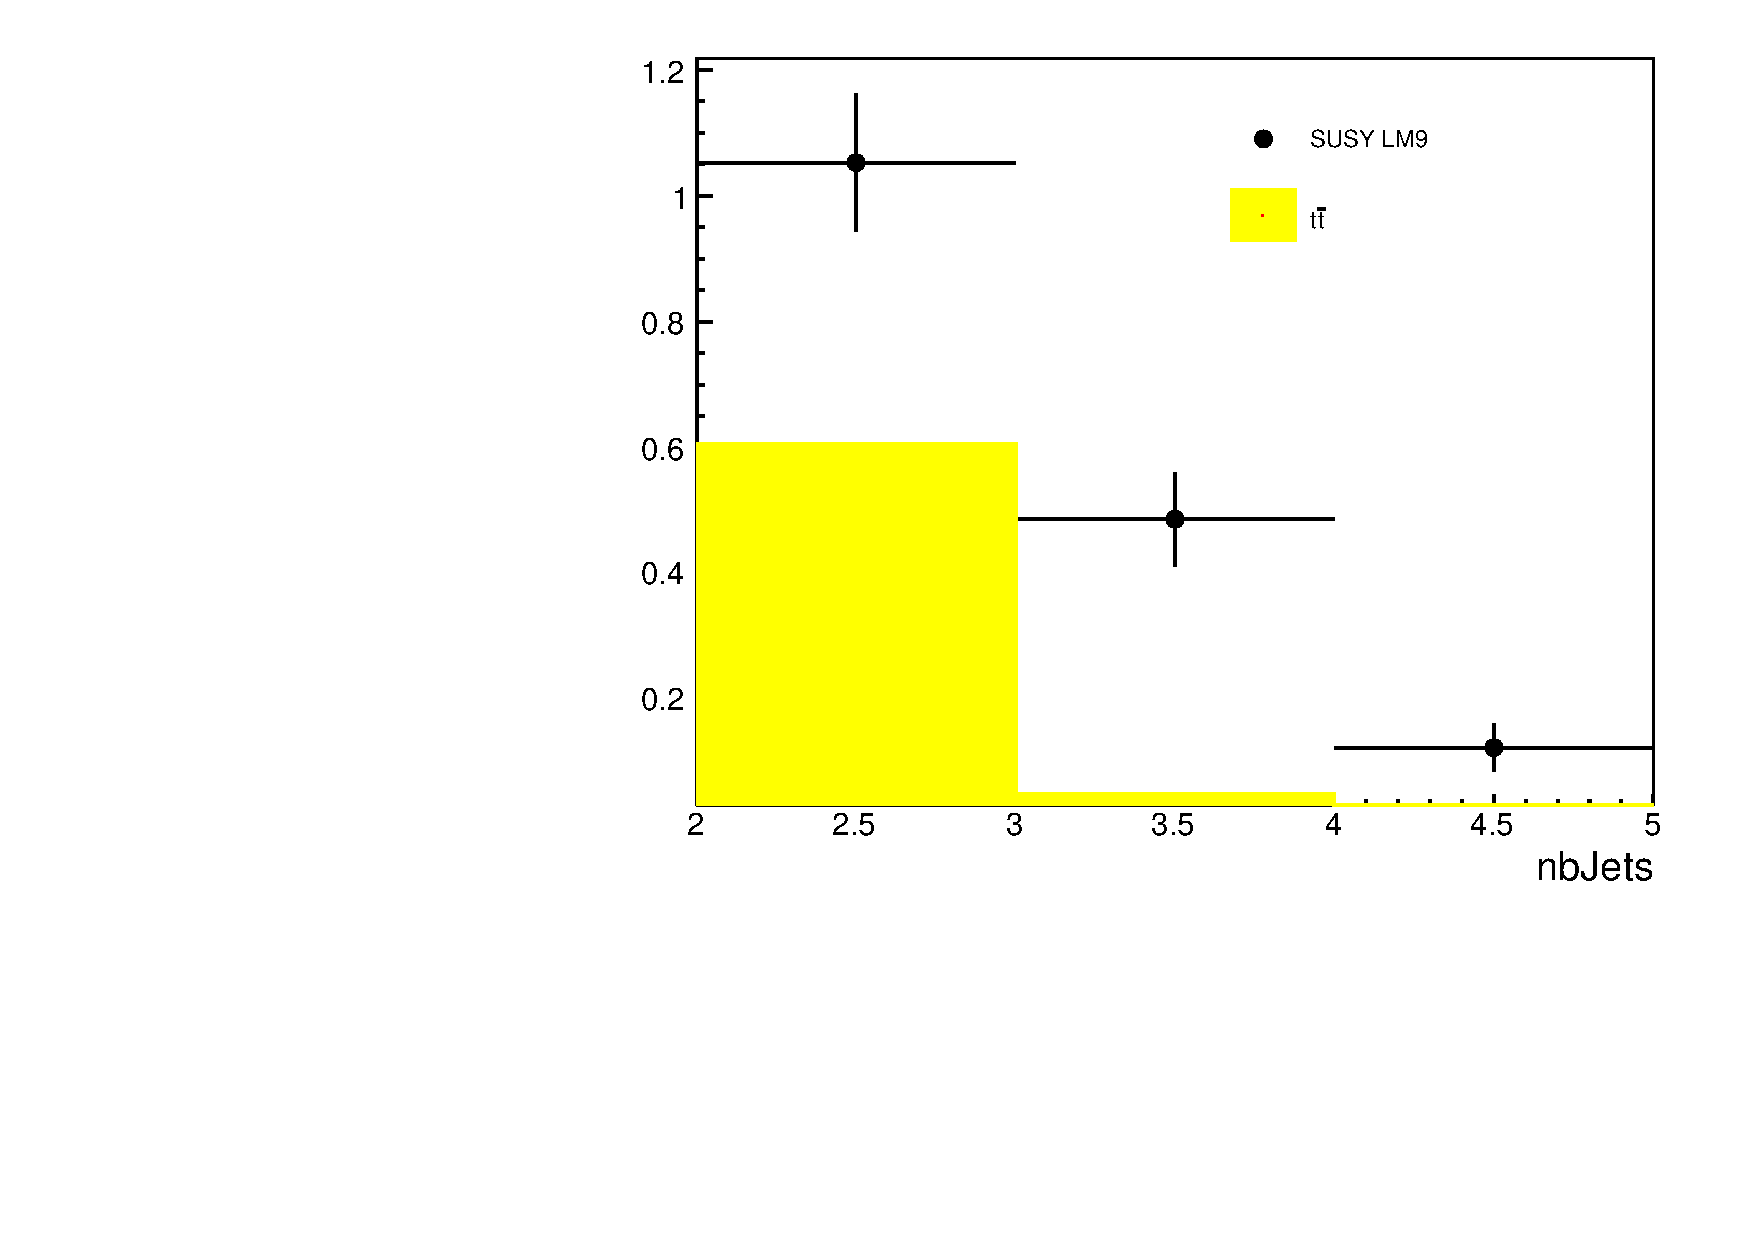
\includegraphics[width=0.48\linewidth, height=0.36\linewidth]{figs/lm9.pdf}
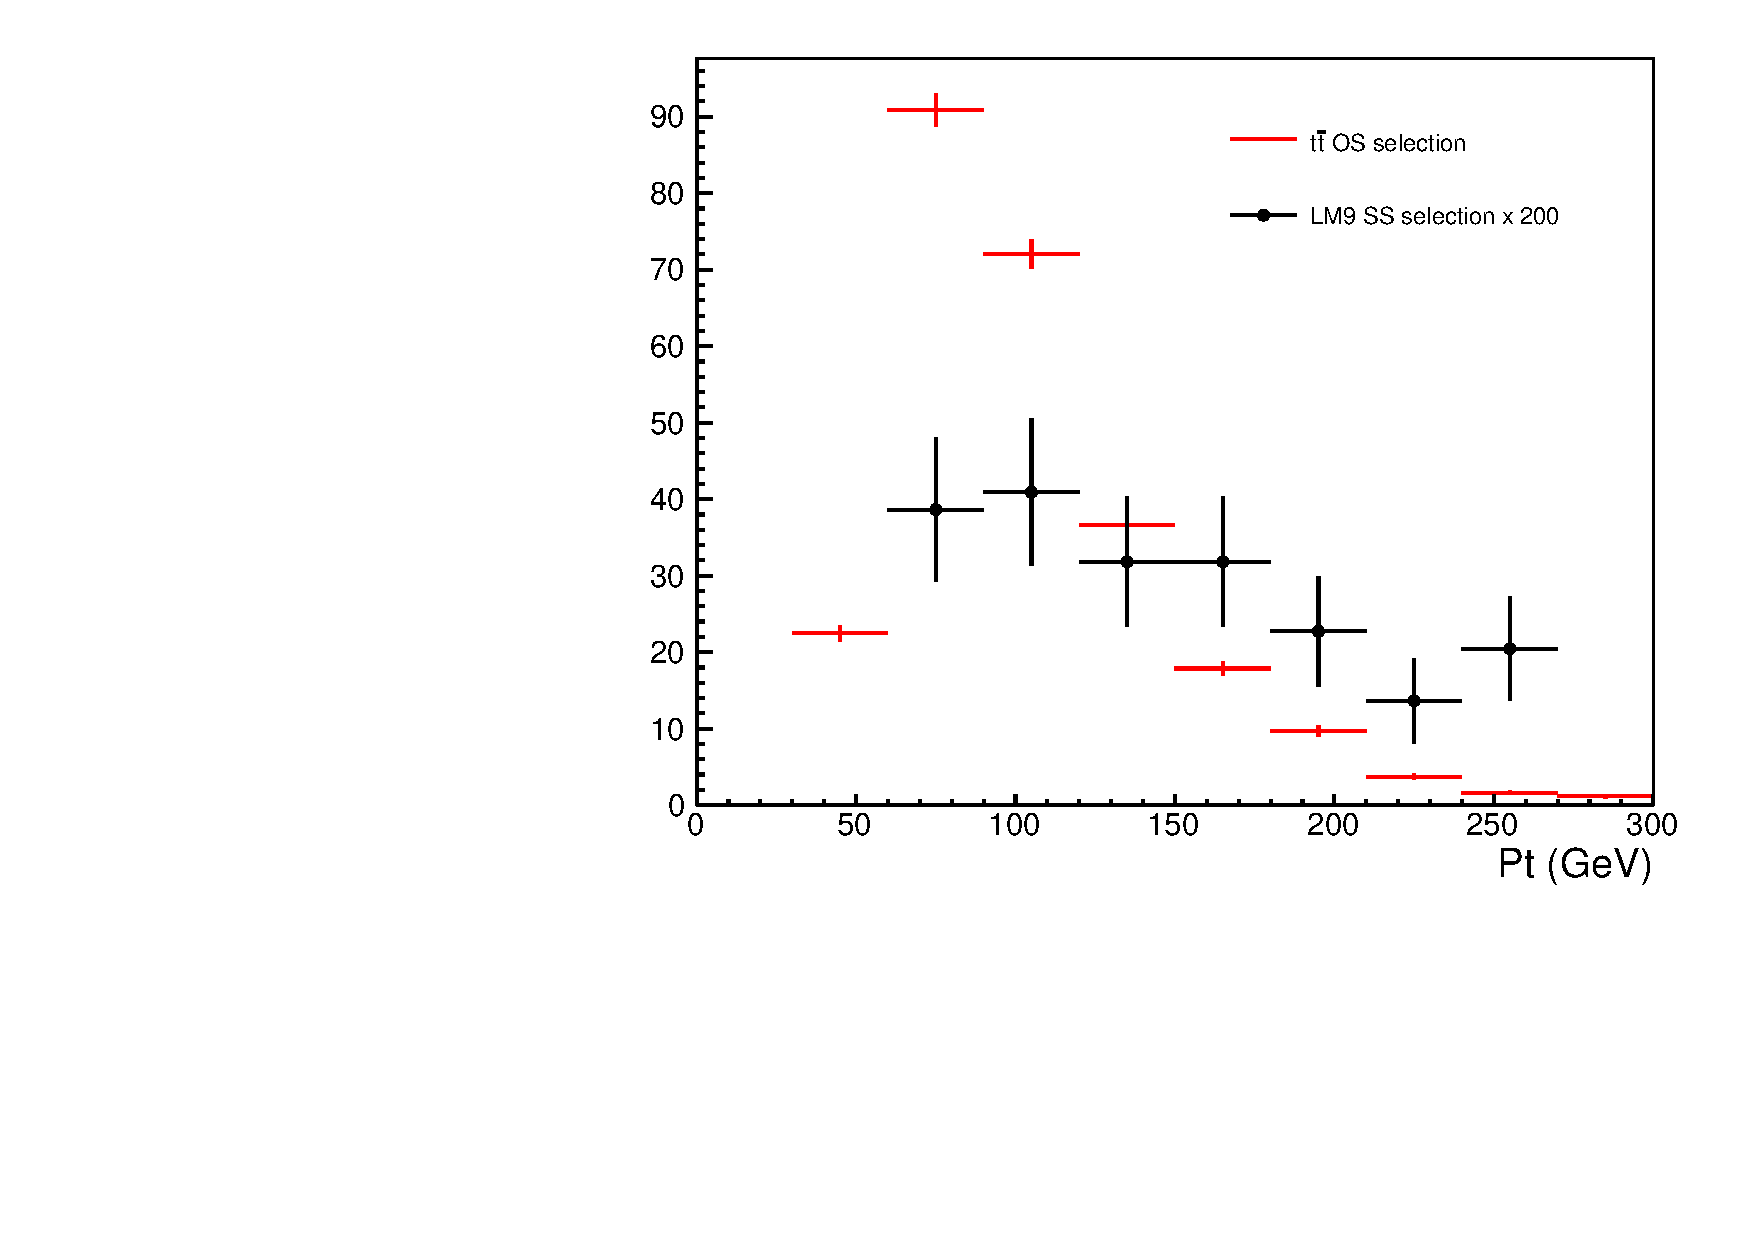
\includegraphics[width=0.6\linewidth, height=0.36\linewidth]{figs/bjetleading.pdf}
\caption{ Differential distributions of leading b-tag jet $p_T$ for the 
LM9 benchmark point and \ttbar\ simulations.
The normalization is arbitraty.\label{fig:lm9ttbar}}
\end{center}
\end{figure}


A summary of systematic uncertainties is given in Table~\ref{tab:systSumm}.
Here the b-tagging systematics is applicable only to the same-sign top production signature.

\begin{table}[h]
\begin{center}
\caption{\small\label{tab:systSumm}Summary of systematic uncertainties on the signal selection and
expectation. 
Reported values are fractional, relative to the total cross section.}
\begin{tabular}{lcccc}\hline
Source 					& $ee$		& $\mu\mu$		& $e\mu$	& all \\ \hline
Lepton selection			& 12\%		& 12\%			& 11\%		& 11\% \\
Energy scale				& 5\%		& 5\%			& 5\%		& 5\% \\
ISR/FSR and PDF				& 2\%		& 2\%			& 2\%		& 2\% 	\\
b-tag selection                         & 10\%          & 10\%                  & 10\%          & 10\% \\
Total without luminosity		& 17\%		& 17\%			& 16\%		& 16\%\\ \hline
Integrated luminosity			& 4.5\%		& 4.5\%			& 4.5\%		& 4.5\%	\\ \hline
Total 					& 17\%	 	& 17\%	 		& 16\% 		& 16\% \\
\hline
\end{tabular}
\end{center}
\end{table}
